\documentclass[12pt]{article}
% add some essential packages, some might not be used

\usepackage[T1]{fontenc}
\usepackage[utf8]{inputenc}
\usepackage[usenames,dvipsnames]{color}
\usepackage{natbib}
\usepackage{authblk}
\usepackage{ragged2e}
\usepackage{amsmath}
\usepackage[a4paper,margin=1in,bottom=1.0in]{geometry}
\usepackage{url}
\usepackage{array}
\usepackage{bbding}
\usepackage{amssymb}
\usepackage{graphicx}  % mini page function
\usepackage{adjustbox}
\usepackage{subcaption}
\usepackage{booktabs}
\usepackage{float}
\usepackage{appendix} % appendix package
\usepackage{hyperref}
\usepackage{url}
\usepackage[english]{babel}
\usepackage{adjustbox}
\usepackage{enumitem}
\usepackage{textgreek}
\usepackage{bibentry}
\nobibliography*
\usepackage{lipsum}


\usepackage{listings}
\usepackage{wasysym}
\usepackage{amsthm}
\usepackage{framed}
\usepackage{bm}
\usepackage{booktabs}  % package for table line
% \usepackage{amsrefs?}  % ams citation style package


\usepackage{rotating} % for the horizontal page table

\usepackage{tikz}
\usetikzlibrary{calc}
\usetikzlibrary{matrix}
\usetikzlibrary{positioning}
\usepackage{color}
\usepackage{setspace}
\usepackage{xcolor}

\usepackage{tcolorbox} % package for making colorful box

 \setlength{\parskip}{0.15cm} % change the paragraph spacing
\renewcommand\labelitemi{$\vcenter{\hbox{\tiny$\bullet$}}$} % set the bullet size as tiny

% \newcommand*\rot{\rotatebox{90}} % for rotate text

\usepackage{sectsty} %package for section size

\sectionfont{\fontsize{14}{12}\selectfont} % Change the section font size

\subsectionfont{\fontsize{13}{12}\selectfont}
\subsubsectionfont{\fontsize{12}{12}\selectfont}

\newcommand\numberthis{\addtocounter{equation}{1}\tag{\theequation}} % new command



\theoremstyle{definition}
\newtheorem{definition}[subsection]{Definition}
\newtheorem{axiom}[subsection]{Axiom}
\newtheorem{example}[subsubsection]{Example}
\newtheorem{theorem}[subsection]{Theorem}
\newtheorem{proposition}[subsection]{Proposition}
\newtheorem{lemma}[subsection]{Lemma}


\usepackage{courier}

% tikzsetting

\usetikzlibrary{shapes,decorations,arrows,calc,arrows.meta,fit,positioning}

\tikzset{
    -Latex,auto,node distance =1 cm and 1 cm,semithick,
    state/.style ={ellipse, draw, minimum width = 0.7 cm},
    point/.style = {circle, draw, inner sep=0.04cm,fill,node contents={}},
    bidirected/.style={Latex-Latex,dashed},
    el/.style = {inner sep=2pt, align=left, sloped}
}

\lstset{language=Python}

\definecolor{mygreen}{rgb}{0,0.6,0}
\definecolor{mygray}{RGB}{145, 153, 165}
\definecolor{mymauve}{rgb}{0.58,0,0.82}

\lstset{
  backgroundcolor=\color{white},   % choose the background color; you must add \usepackage{color} or \usepackage{xcolor}; should come as last argument
  basicstyle=\footnotesize,        % the size of the fonts that are used for the code
  breakatwhitespace=false,         % sets if automatic breaks should only happen at whitespace
  breaklines=true,                 % sets automatic line breaking
  captionpos=b,                    % sets the caption-position to bottom
  commentstyle=\color{gray},    % comment style
  deletekeywords={...},            % if you want to delete keywords from the given language
  escapeinside={\%*}{*)},          % if you want to add LaTeX within your code
  extendedchars=true,              % lets you use non-ASCII characters; for 8-bits encodings only, does not work with UTF-8
  frame=single,	                   % adds a frame around the code
  keepspaces=true,                 % keeps spaces in text, useful for keeping indentation of code (possibly needs columns=flexible)
  keywordstyle=\color{RoyalBlue},       % keyword style
  language=Python,                 % the language of the code
  morekeywords={*,...},            % if you want to add more keywords to the set
  numbers=left,                    % where to put the line-numbers; possible values are (none, left, right)
  numbersep=5pt,                   % how far the line-numbers are from the code
  numberstyle=\tiny\color{gray}, % the style that is used for the line-numbers
  rulecolor=\color{black},         % if not set, the frame-color may be changed on line-breaks within not-black text (e.g. comments (green here))
  showspaces=false,                % show spaces everywhere adding particular underscores; it overrides 'showstringspaces'
  showstringspaces=false,          % underline spaces within strings only
  showtabs=false,                  % show tabs within strings adding particular underscores
  stepnumber=2,                    % the step between two line-numbers. If it's 1, each line will be numbered
  stringstyle=\color{mymauve},     % string literal style
  tabsize=2,	                   % sets default tabsize to 2 spaces
  title=\lstname                   % show the filename of files included with \lstinputlisting; also try caption instead of title
}

\numberwithin{equation}{section}
\numberwithin{figure}{section}
\numberwithin{table}{section}


% Define colors
\definecolor{cmd}{HTML}{F7F7F9}
\DeclareMathOperator{\di}{d\!}

\newcommand{\pr}{$\mathbb{P}$}
\newcommand{\pre}{\mathbb{P}}

\begin{document}

\title{Gradient Descent for Risk Optimization}
\author{Michael}
\date{}
\maketitle

\section{Intuition Behind Gradient Descent}

Although the term `gradient descent' is very fancy, the idea and intuition behind this term is extremely simple. It is same for \textit{convergence rate}. All you need to know is that what is the meaning of derivative.

The \textbf{derivative} of a function of a real variable measures the sensitivity to change of the function value (output value) with respect to a change in its argument (input value). Let's draw a table for this definition.
\begin{table}[H]
  \centering
  \caption{Derivative}
  \begin{tabular}{lcc}
    \hline
    Measures & Input value & Output value \\
    \hline
    Sensitivity to & Change & Change \\
    \hline
    $\downarrow$ & $\downarrow$ & $\downarrow$ \\
    & change rate & change rate \\
    & $\downarrow$ & $\downarrow$ \\
    \hline
    \multicolumn{3}{c}{Convergence Rate} \\
    \hline
  \end{tabular}
\end{table}

If you got the idea of table 1.1, you can stop reading the section 1 and jump to section 2 and 3. If not, allow me to spend a little more time to explain this.
\begin{figure}[H]
  \centering
  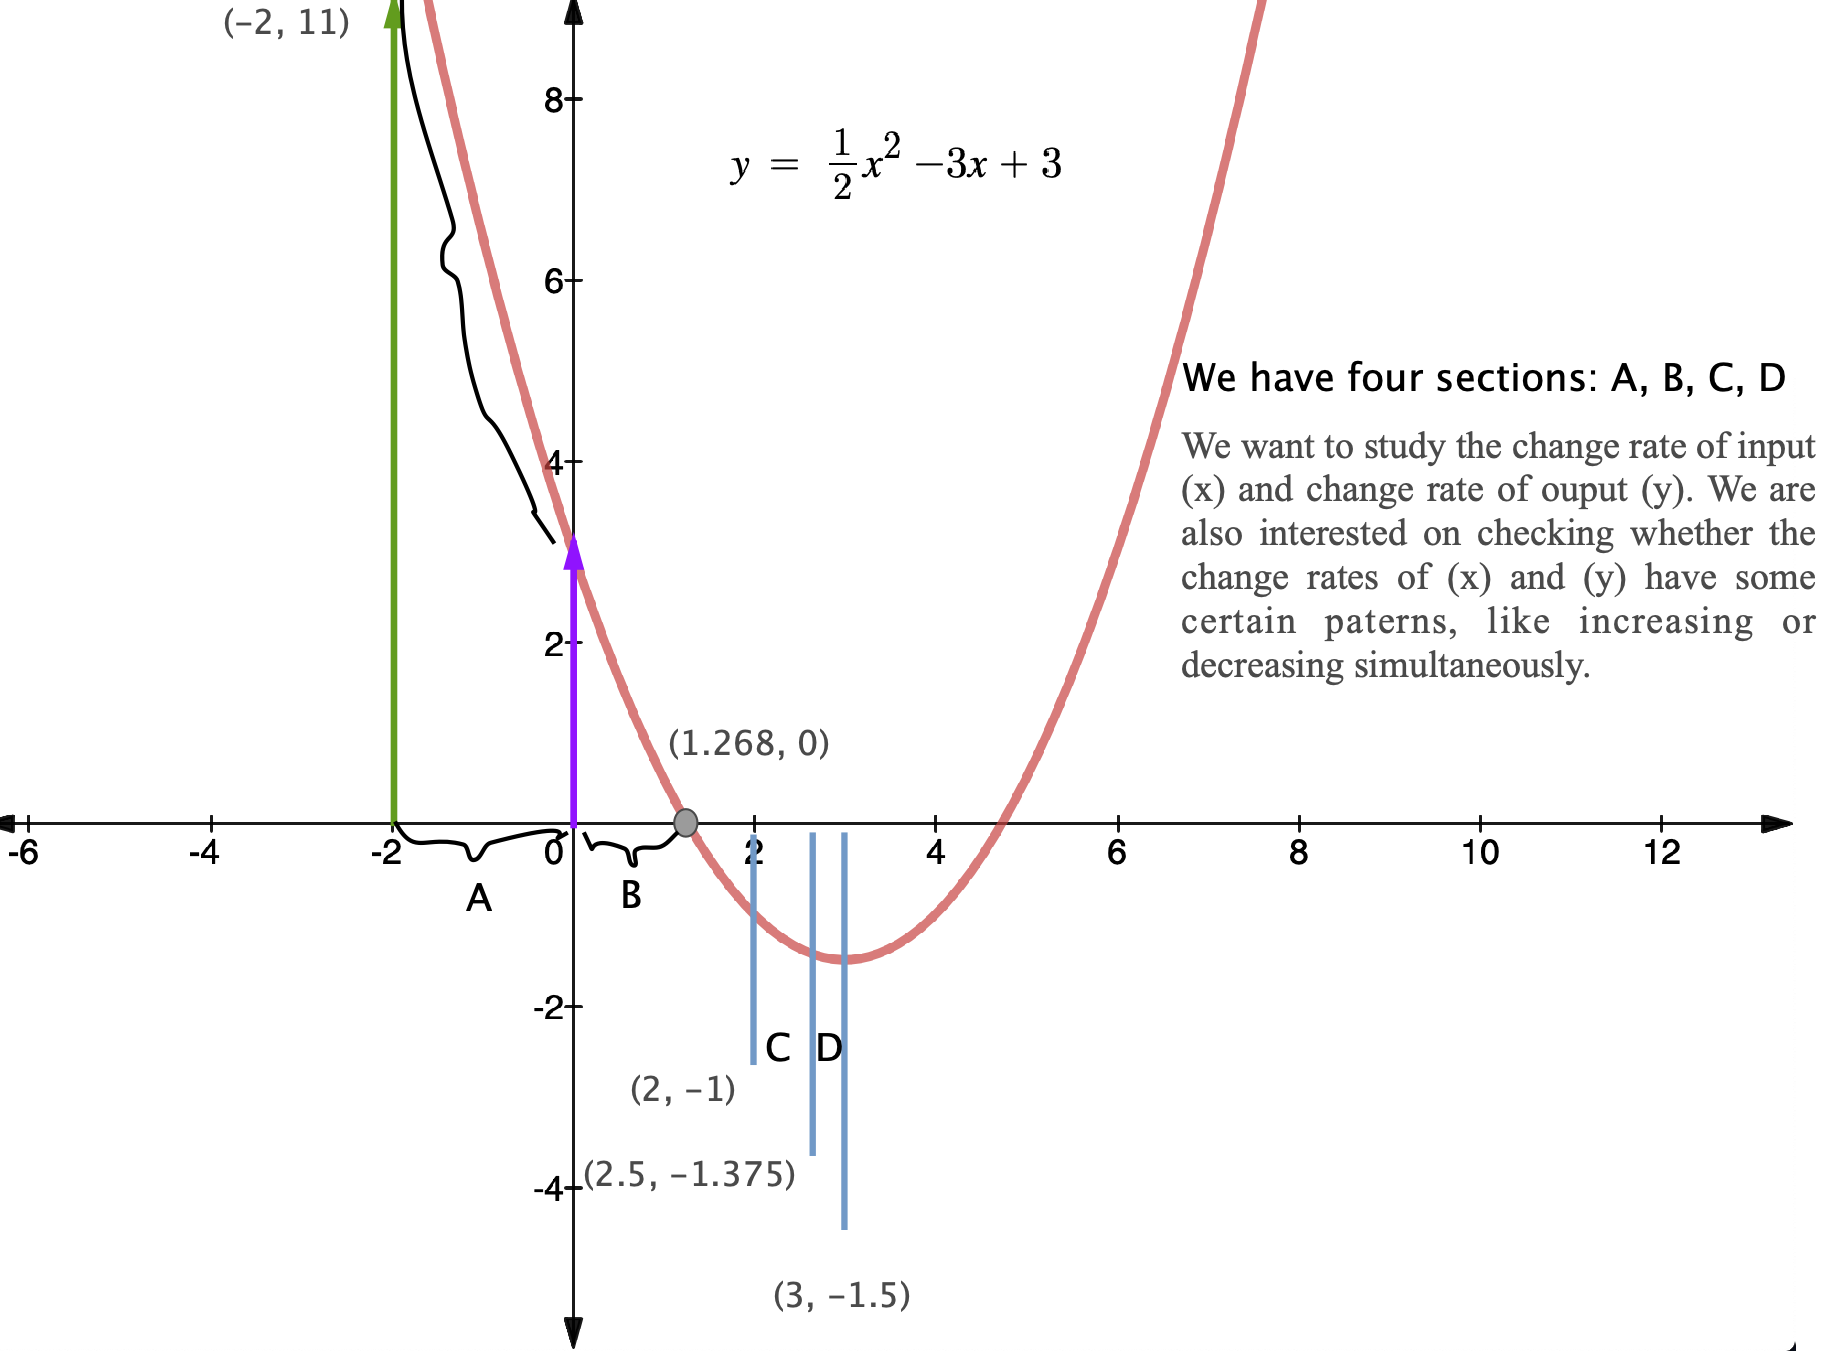
\includegraphics[width=0.7\textwidth]{gradientEg}
  \caption{Gradient Visualisation}
\end{figure}

Again, the derivative is not just about the measurement of change of input and output, it also reflects the sensitivity of those changes. Take a look the figure 1.1, tell me where both input ($x$) and output ($y$) are changing fast, and where both input ($x$) and output ($y$) are changing slowly\footnote{If we assume that speed of changing is measured by the difference between two values.}.

From the figure 1.1, we can see that in section A, both input ($x$) and output ($y$) are changing quite fast by measuring the differences. When it comes to section C and D, the changing rates for input-$x$ and output-$y$ are decreasing simultaneously. We also say that input $x$ and output $y$ have the same \textbf{convergence rate} intuitively\footnote{This is not formal mathematical definition.}. For the \textbf{supervised learning} in \textit{machine learning}, it starts to do optimization with the tool of convergence rate.

Now, let's check the formal definition of derivative. The slope $m$ of the secant line is the difference between the y values of these points divided by the difference between the x values, that is,
\begin{align*}
  m = \frac{\Delta f(x)}{\Delta x} = \frac{f(x+h) - f(x)}{(x+h) -x} = \frac{f(x+h)-f(x)}{h}
\end{align*}
Geometrically, the limit of the secant lines is the tangent line. Therefore, the limit of the difference quotient as $h$ approaches zero, if it exists, should represent the slope of the tangent line to $(x, f(x))$. This limit is defined to be the derivative of the function $f$ at $x$:
\begin{align*}
  f'(x) = \lim_{h\to 0} \frac{f(x+h) - f(x)}{h}
\end{align*}

With the riview of defintion of derivative, we are ready to apply the so called \textbf{gradient descent} algorithm to find the minimum of a function.
\begin{definition}
  Gradient descent is a first-order iterative optimization algorithm for finding the minimum of a function.
\end{definition}

Let's disentangle the convergence rate for the function $y= \frac{1}{2}x^2 - 3x + 3$ in figure 1.1 by presenting the following figure and table:
\begin{figure}[H]
  \centering
  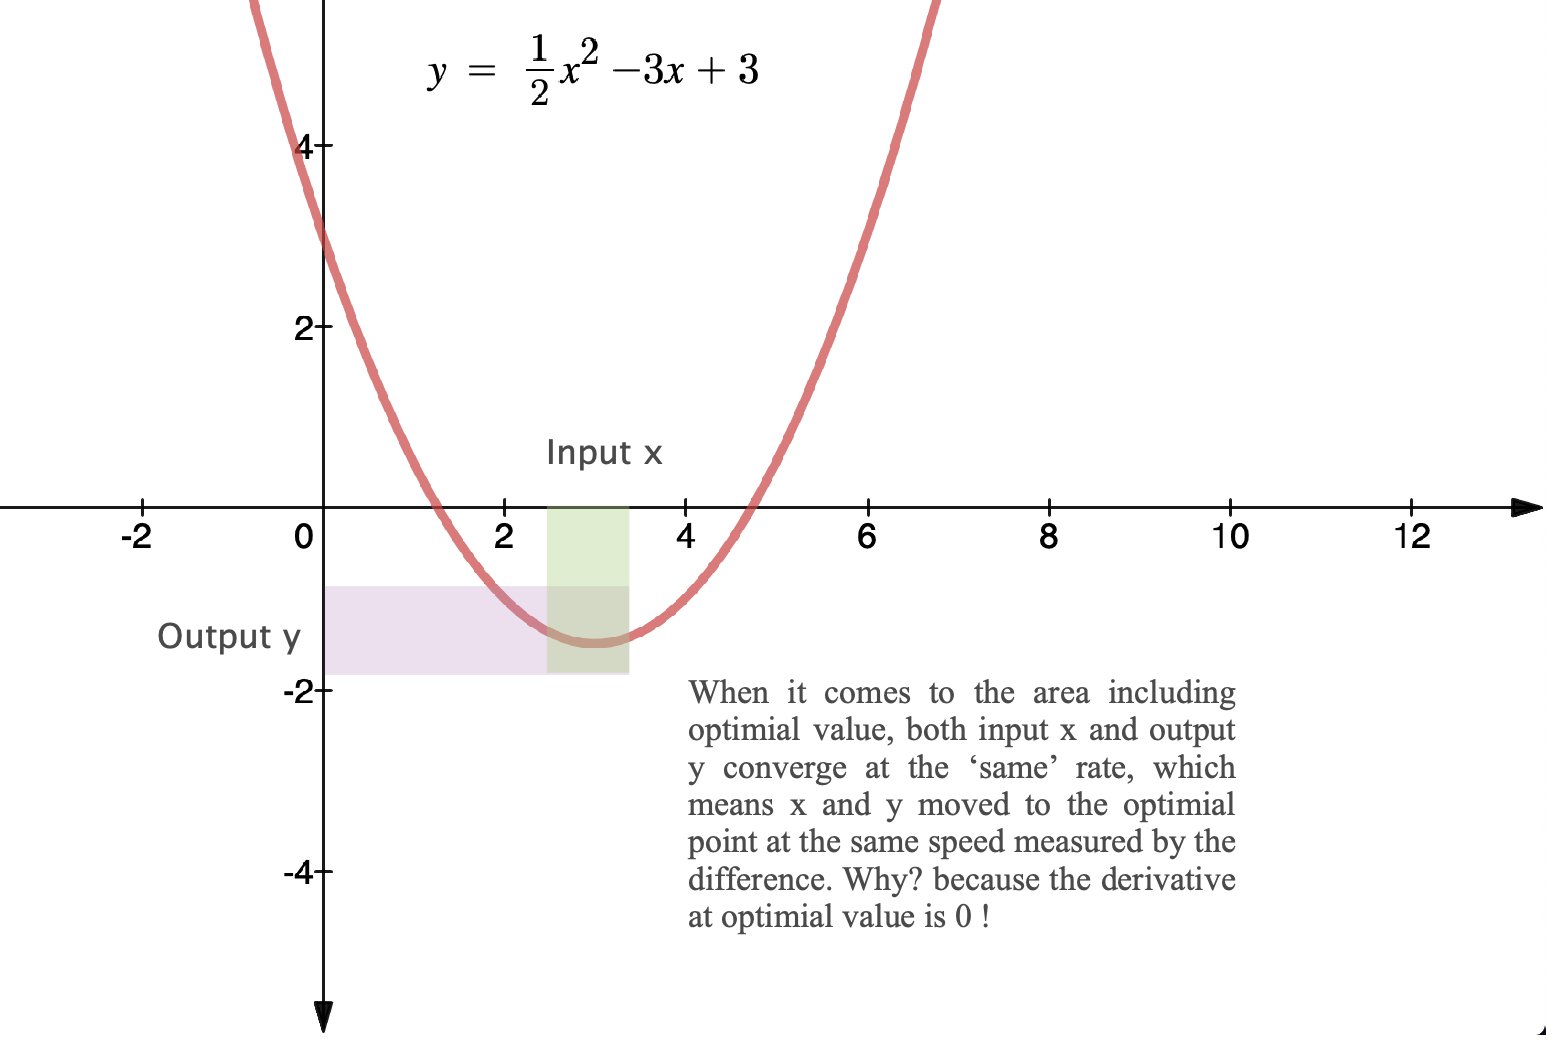
\includegraphics[width = 0.7 \textwidth]{gradientEg2}
\end{figure}
{\footnotesize
\begin{table}[H]
  \centering
  \caption{Show the gradient descent step by step}
  \begin{tabular}{lcccc}
    \hline
    \hline
    Section & Points & Change of input($x$) & Change of ouput ($y$) & Convergence ratio  \\
    \hline
    A & $(-2, 11)$ & \\
    & $(0,0)$ & 2 & 11 & $11/2 = 5.5$ \\
    \hline
    B & $(0,0)$ & \\
    & $(2, $-$1)$ & 2 & 1 & $1/2 = 0.5$ \\
      \hline
    C & $(2, $-$1)$ &  \\
    & $(2.5, $-$1.375)$ & 0.5 & 0.375 & $0.375/0.5 = 0.75$ \\
    \hline
    D & $(2.5, $-$1.375)$ & \\
    & $(3, $-$1.5)$ & 0.5 & 0.125 & $0.125/0.5 = 0.25$ \\
    \hline
    \multicolumn{5}{c}{$\cdots$} \\
    \hline
    & $(2.9, $-$1.49499)$& \\
    & $(2.95, $-$1.49875)$ & 0.05 & 0.00376 & $0.00376 /0.05 = 0.075$  \\
    \hline
    \multicolumn{5}{c}{$\cdots$} \\
    \hline
    & $(2.98, $-$1.499799)$& \\
    & $(2.99, $-$1.499950)$ & 0.01 & 0.000151 & $0.00376 /0.05 = 0.00151$  \\
    \hline
    \multicolumn{5}{c}{we have learning rate $\alpha$ to scale the convergence rate = 1} \\
    \hline
  \end{tabular}
\end{table}
}

\textbf{Markup:} it's all about simultaneous moving of input ($x$) and ($y$).

\section{A Mathematical example}

Now, we will employ the gradient descent\footnote{Review the definition, it's an algorithm.} to find the minimum value for the function in section 1:
\begin{align*}
  f(x) = \frac{1}{2} x^2 - 3x + 3
\end{align*}

The intuition of using gradient descent is that we are trying to iterate the change rate of input $x$ by tracing the change rate of output $y$. To do this, we need the help from the derivative of the function. Here is the Python code:
\begin{lstlisting}[caption = Gradient Descent Math Example]
  # Gradient Descent: mathematical example
  # @ Michael


  # define function
  def qudraticfun(x):
      y = 1/2 * x**2 - 3 * x + 3
      return(y)


  # define the derivative
  def qudraticder(x):
      yprime = x - 3
      return(yprime)


  # find the minium numerically

  update_x = 0  # most time we start it from zero
  alpha = 0.01  # learning rate
  tolerate_rule = 1  # initialize the tolerate rule for stopping iterating
  max_iters = 10000  # set the maximum iterative number

  i = 0  # interation counting index
  while tolerate_rule >= 0.00001 and i <= max_iters:
      start_x = update_x  # set the starting value
      update_x = start_x - alpha * qudraticder(start_x)
      tolerate_rule = abs(update_x - start_x)

  print("The minimum value is", qudraticfun(update_x),
        "when x is equal to", update_x)

  # The minimum value is -1.4999995136117308 when x is equal to 2.999013705653870
\end{lstlisting}

\section{A Machine Learning Example}

For most students who have done econometric 101 or statistics 101, least squares estimation (LSE) and maximum likelihood estimation (MLE) are not unusual. Later, we can show that LSE and MLE are just one of special cases among gradient descent methods. In the section, we will apply gradient descent for the linear regression in one variable. Then the multivariable cases will be given. All examples are from \cite{ng2014cs229}, unless otherwise stated.

Unlike the mathematical example in section 2, we do not have the given function to optimize. Therefore, we need define the function for doing optimization. In machine learning, this function is called the \textbf{cost function} or \textbf{loss function}. In machine learning, we still have \textit{input} and \textit{output} like in the following table:
\begin{table}[H]
  \centering
  \caption{Input and Output of Machine Learning}
  \begin{tabular}{lcc}
    \hline
    \hline
    Input & Function &Output  \\
    \hline
    Training data $X$ & Regression or Classification & Estimated coefficients $\theta$\\
    Matrix form & & Vector or matrix  \\
    \hline
    Measure & \multicolumn{2}{c}{convergence rate between $\theta$ and loss function} \\
    \hline
  \end{tabular}
\end{table}

We will use \texttt{Ex1data.csv} to run one variable regression. The first column is the population of a city and the second column is the profit of a food truck in that city. A negative value for profit indicates a loss. The first column refers to the population size in 10,000s and the second column refers to the profit in \$10,000s.
\begin{table}[H]
  \centering
  \begin{tabular}{c|c|c}
  Row Index  & Population	& Profit \\
    \hline
0	&6.1101 &	17.5920 \\
1	&5.5277&	9.1302 \\
2	&8.5186&	13.6620 \\
3	&7.0032	&11.8540 \\
4	&5.8598&	6.8233 \\
$\vdots$ & \\
\hline
  \end{tabular}
\end{table}

Now, we must decide how we are going to represent the regression function $f$. As an initial choice, let's say we decide to approximate $y$ as a linear function of $x$:
\begin{align}
  f(x) = \theta_0 + \theta_1 x
\end{align}
Here, the $\theta_i$'s are the \textbf{parameters} (also called \textbf{weights}). In this function, we set $x_0 = 1$ to make the intercept become $\theta_0$. Okay, how to we find the optimal parameters $\theta$? We need fist set the cost (loss) functions, and then choose $\theta$ to minimize the cost (loss) functions.

There are several loss (cost) functions we can use. Here is the list:
\begin{enumerate}[label=(\roman*)]
  \item Squared Error Loss: $\frac{1}{2}[y - f(x)]^2$
  \item Absolute Error Loss: $|y - f(x)|$
  \item Huber's Loss: $\begin{cases}
    & \frac{1}{2}[y - f(x)]^2 \ \ if |y - f(x)| \leq \delta \\
    & \delta[|y - f(x)| - \frac{1}{2} \delta] \ \  otherwise
  \end{cases}$
\end{enumerate}

Let's use the squared error loss function, which we can write it as
\begin{align}
  J(\theta) = \frac{1}{2} \sum_{i=1}^n [f(x^i) - y^i]^2
\end{align}
where $n$ is the length of dataset or size of vector $y$ (or $x$). Our task is to minimize the equation (3.2). If you have read the section 2 carefully, then you will realise that the first step is to write down it's derivative:
\begin{align*}
  \frac{\partial }{\partial \theta_j} J(\theta)& = \frac{\partial }{\partial \theta_j} \frac{1}{2} \sum_{i=1}^n [f(x^i) - y^i]^2 \\
  & = 1 \cdot \frac{1}{2}\sum_{i=1}^n [f(x) - y] \frac{\partial }{\partial \theta_j}  [f(x) - y] \tag{chain rule}
\end{align*}

Now, substitute equation (3.1) into the above general case, we can have:
\begin{align}
  \frac{\partial }{\partial \theta_0} J(\theta)& = [f(x) - y] \theta_0 \\
  \frac{\partial }{\partial \theta_1} J(\theta)& = [f(x) - y] \theta_1
\end{align}

Then we can apply the gradient descent with derivative in equation (3.3) and (3.4) to update the parameters:
\begin{align}
  \theta_j = \theta_j - \alpha \sum_{i=1}^n [f(x) -y] \theta_j \ \ \ \ \text{(for every j)}
\end{align}

Does the equation (3.5) looks familiar to you? It should be if you have done the python code in listing 1 (page 4). The following is the regression code with gradient descent.

\begin{lstlisting}[caption = Gradient Descent Regression]
  # Gradient descent: regression example
  # @ Michael

  import pandas as pd
  import numpy as np
  import os
  import matplotlib.pyplot as plt


  # check the working directory
  os.getcwd()
  os.chdir('/Users/Michael/Documents/MachineLearning/GraidentDescent')

  # read the dataset
  ex1data = pd.read_csv('Ex1data.csv', names=['Population', 'Profit'])

  # explore the dataset
  ex1data.head()
  ex1data.columns
  ex1data.shape  # (97, 2)

  fig, ax = plt.subplots(figsize=(6, 5))
  ax.scatter(ex1data.Population, ex1data.Profit, marker='x')
  ax.set(xlabel='Population of City in 10,000s',
         ylabel='Profit in $10,000s',
         title='Plot of X and Y')
  fig.show()


  # run regression: use population to predict profit

  # set x
  datamatrix = np.asmatrix(ex1data['Population']).transpose()
  datamatrix.shape
  input_x = np.hstack([np.ones(ex1data.shape[0]).reshape(-1, 1), datamatrix])
  input_x.shape  # check the matrix shape, (97, 2)
  input_y = np.asmatrix(ex1data.Profit).transpose()
  input_y.shape


  # define the loss function
  def SquareLoss(x, y, theta):
      """
      A square error loss function to compare the loss (cost) error
      Input: x - matrix n by m
             y - vector n by 1
             theta - vector m by 1, order matters considering the intercept
      Output: the sum of squared error
      """
      n = x.shape[0]
      fx = x @ theta  # matrix (dot) production
      loss = 1/2 * 1/n * np.sum(np.square(fx - y))  # use average with 1/n

      return(loss)


  # set intial theta value
  theta_initial = np.array([0, 0]).reshape(-1, 1)
  # test SquareLoss function
  SquareLoss(input_x, input_y, theta_initial)  # 32.072733877455676


  # define the gradient descent function
  def GradientDescent(x, y, theta, alpha, tolerate, maxiterate):
      i = 0  # set the iteration counting index
      tolerate_rule = 1  # set the initial tolerate rate
      n = x.shape[0]
      current_theta = theta
      cost_vector = np.empty([0, 1])

      # iterate
      while tolerate_rule >= tolerate and i <= maxiterate:
          sl = np.array(SquareLoss(x, y, current_theta)).reshape([1, 1])
          cost_vector = np.append(cost_vector, sl, axis=0)  # store cost function
          fx = x @ current_theta
          update_theta = current_theta - alpha * (1/n) * x.transpose() @ (fx - y)
          tolerate_rule = np.min(np.abs(update_theta - current_theta))
          i += 1
          current_theta = update_theta

      return(current_theta, cost_vector)


  theta_initial = np.array([0, 0]).reshape(-1, 1)  # give initial value
  alpha = 0.01  # learning rate
  tolerate = 0.00001  # tolerate rates
  maxiter1 = 1500
  coefficents1, lossvalues1 = GradientDescent(input_x, input_y,
                                              theta_initial, alpha,
                                              tolerate, maxiter1)

  print("The estimated coefficients are", coefficents1)
  # The estimated coefficients are [[-3.63077001] [ 1.16641043]]
  lossvalues1.shape
  # iteration stops because function reaches to maxiter, (1501, 1)
  plt.plot(lossvalues1[1:])

  # we can set maxiter = 3000 to see what's going on
  theta_initial = np.array([0, 0]).reshape(-1, 1)  # give initial value
  alpha = 0.01  # learning rate
  tolerate = 0.00001  # tolerate rates
  maxiter2 = 3000
  coefficents2, lossvalues2 = GradientDescent(input_x, input_y,
                                              theta_initial, alpha,
                                              tolerate, maxiter2)

  print("The estimated coefficients are", coefficents2)
  # The estimated coefficients are [[-3.84072806][ 1.18750299]]


  lossvalues2.shape  # (2372, 1), iteration stops because of tolerate

  # plot the cost function
  fig, ax = plt.subplots(figsize=(6, 5))
  ax.plot(lossvalues2[1:])
  ax.set(title='Plot of Loss Function', xlabel='Iteration',
         ylabel='Loss')
  fig.show()


  # plot the regression line
  xdomain = np.linspace(5, 25)
  yfit = coefficents2[0] + coefficents2[1] * xdomain

  fig, ax = plt.subplots(figsize=(6, 5), sharex=True)
  ax.scatter(ex1data.Population, ex1data.Profit, marker='x',
             label='Raw data')
  ax.plot(xdomain.reshape(-1, 1), yfit.reshape(-1, 1), 'r',
          label='Linear regression (Gradient descent)')
  ax.set(xlabel='Population of City in 10,000s',
         ylabel='Profit in $10,000s',
         title='Plot of X and Y with fitted regression')
  ax.legend(loc=4)
  fig.show()


  # show the dynamics of loss function in gradient descent
  # I will add it later
  # End of code
\end{lstlisting}






















\newpage
\bibliography{/Users/Michael/Documents/MachineLearning/ML.bib}
\bibliographystyle{apalike}
\end{document}
